\chapter{Recommendations for future work}

\section{Bleeding-edge LLMs}
As originally mentioned in the literature review, the LLM space is rapidly expanding and continued to do so even throughout this project's 
development. Throughout the main development process, the best identified model in terms of performance to cost was gpt-4o-mini. However,
OpenAI has since gone on to release more intelligent models at similar price points, namely gpt-4.1-mini, and gpt-4.1-nano. The 4.1 mini model 
is 2.6x more expensive than 4o-mini (\$0.40/1M input tokens) \autocite{openaiPricingOpenAIAPI}, 
though its benchmark scores are only slightly lower than the full gpt-4o model for a fraction of its cost (\$2.50/1M input tokens). 

\begin{figure}[H]
    \centering
    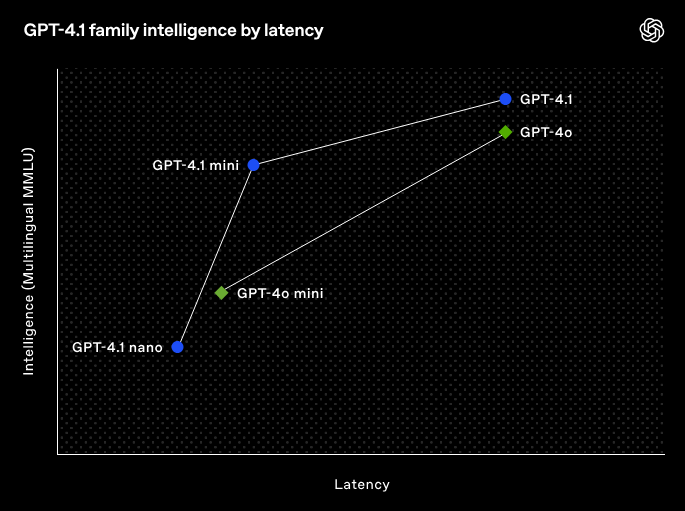
\includegraphics[width=.75\textwidth]{Conclusion and Future/GPT4.1.png}
    \caption{A relative performance chart of GPT models on the MMLU benchmark \autocite{openaiIntroducingGPT41API}.\label{fig:GPT41Perf}}
\end{figure}

\noindent gpt-4.1-nano is observed to have lower performance than 4o-mini, though this is also reflected in its extremely low latency and 
50\% reduced cost of only \$0.10 per million tokens. The full GPT-4.1 model is shown to be extremely intelligent according to OpenAI's graph,
though its pricing is simply too high in the scope of this project (\$2/1M input tokens, \$8/1M output tokens).

\para In summary, it would likely be beneficial for future similar works to utilise the latest developments in the LLM space, and remain observant 
of upcoming releases to capitalise as soon as they become available.

\section{Agentic RAG}
While the produced chatbot was able to answer the majority of questions correctly, it is possible that the implementation of an agentic RAG 
solution could have enhanced its results even further through an iterative corrective RAG cycle of answer evaluation. 
This was attempted during development, though repeatedly proved unsuccessful in this specific use case. 
To avoid jeopardising the overall project schedule, it was therefore not present in the final product. 

\para Therefore, future similar works should plan extensively ahead of time for how they could implement such a solution to ensure maximum 
answer accuracy. However, they should be mindful that the latency will greatly increase if the chatbot repeatedly deems its own answers 
to be incorrect, and users may perceive this as a system failure.

\section{User feedback}
Uncontrollable external circumstances meant that user feedback could not be gathered at key stages throughout the product's iterative 
development cycle, with key observations such as those recorded in Chapter \ref{ch:Evaluation} being performed single-handedly.
This is a key element of the Agile development process, and the failure to do so likely had negative consequences on the final product.

\para As such, any future works should always endeavour to obtain constant user feedback to ensure their work is of a constant 
good standard.

% \section{Multi-purposing}
% The framework used to build the chatbot does not entirely limit it to specifically being BCU-related. It is possible that future works 
% could implement their own PDF embedder as part of the frontend UI to turn the chatbot from answering questions only on BCU to answering 
% questions based on any given PDF.